\documentclass[tikz,border=8pt]{standalone}
\usepackage{amsmath,amssymb}
\usetikzlibrary{arrows.meta,automata,positioning,quotes}
\begin{document}
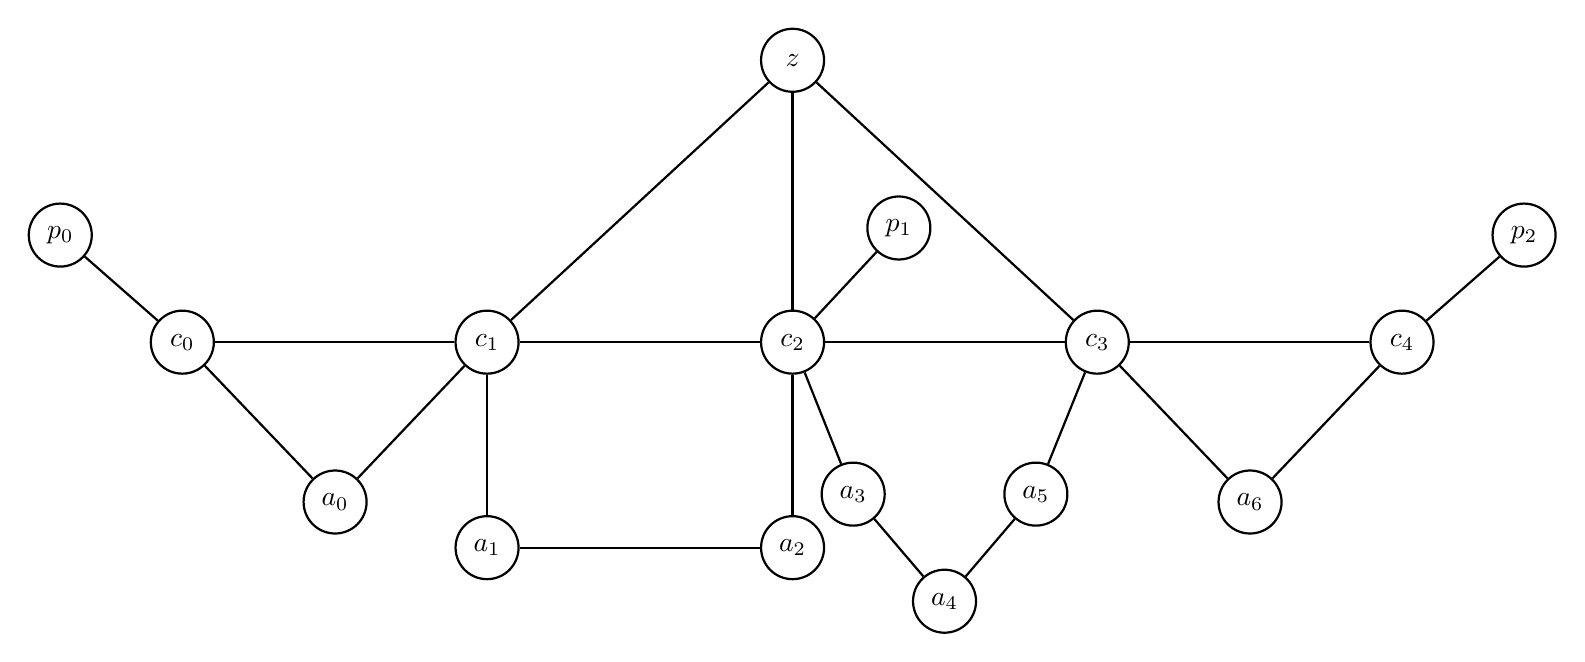
\begin{tikzpicture}[x=1cm,y=1cm]
\tikzset{
  graphnode/.style={circle,draw,thick,minimum size=8mm,inner sep=1pt,font=\sffamily},
  directed/.style={-{Stealth[length=2.4mm]},thick},
  undirected/.style={thick}
}
\node[graphnode] (n_c0) at (-1.04,0.07) {$c_0$};
\node[graphnode] (n_c1) at (2.83,0.07) {$c_1$};
\node[graphnode] (n_c2) at (6.71,0.07) {$c_2$};
\node[graphnode] (n_c3) at (10.58,0.07) {$c_3$};
\node[graphnode] (n_c4) at (14.45,0.07) {$c_4$};
\node[graphnode] (n_a0) at (0.90,-1.96) {$a_0$};
\node[graphnode] (n_a1) at (2.83,-2.54) {$a_1$};
\node[graphnode] (n_a2) at (6.71,-2.54) {$a_2$};
\node[graphnode] (n_a3) at (7.48,-1.86) {$a_3$};
\node[graphnode] (n_a4) at (8.64,-3.22) {$a_4$};
\node[graphnode] (n_a5) at (9.80,-1.86) {$a_5$};
\node[graphnode] (n_a6) at (12.52,-1.96) {$a_6$};
\node[graphnode] (n_p0) at (-2.59,1.43) {$p_0$};
\node[graphnode] (n_p1) at (8.06,1.52) {$p_1$};
\node[graphnode] (n_p2) at (16.00,1.43) {$p_2$};
\node[graphnode] (n_z) at (6.71,3.65) {$z$};
\draw[undirected] (n_c0) -- (n_a0);
\draw[undirected] (n_a0) -- (n_c1);
\draw[undirected] (n_c1) -- (n_c0);
\draw[undirected] (n_c1) -- (n_a1);
\draw[undirected] (n_a1) -- (n_a2);
\draw[undirected] (n_a2) -- (n_c2);
\draw[undirected] (n_c2) -- (n_c1);
\draw[undirected] (n_c2) -- (n_a3);
\draw[undirected] (n_a3) -- (n_a4);
\draw[undirected] (n_a4) -- (n_a5);
\draw[undirected] (n_a5) -- (n_c3);
\draw[undirected] (n_c3) -- (n_c2);
\draw[undirected] (n_c3) -- (n_a6);
\draw[undirected] (n_a6) -- (n_c4);
\draw[undirected] (n_c4) -- (n_c3);
\draw[undirected] (n_c0) -- (n_p0);
\draw[undirected] (n_c2) -- (n_p1);
\draw[undirected] (n_c4) -- (n_p2);
\draw[undirected] (n_z) -- (n_c1);
\draw[undirected] (n_z) -- (n_c2);
\draw[undirected] (n_z) -- (n_c3);
\end{tikzpicture}
\end{document}
